\documentclass[../main.tex]{subfiles}
\graphicspath{{\subfix{..}}}
\begin{document}
\chapter{Calculation of optimal $\alpha$ for estimator combination}
\label{sec:annex:jcnn:alpha}

This annex the details of the determination of the optimal $\alpha$ for estimator combination presented in section \ref{sec:jcnn:combination}.

As a reminder, the combine estimator $\hat{\theta}$ of $X$ is defined as
\begin{equation}
  \hat{\theta}(X) = \alpha \theta_N + (1 - \alpha) \theta_C; ~ \alpha \in [0; 1]
\end{equation}
where $\theta_N$ and $\theta_C$ are both estimator of X.

\section{Unbiased estimator}
For the unbiased estimator, it is straight-forward. We search $\alpha$ such as $E[\hat{\theta}] = X$
\begin{align}
  E[\hat{\theta}] &= E[\alpha \theta_N + (1-\alpha) \theta_C] \\
                  &= E[\alpha \theta_N] + E[(1-\alpha) \theta_C] \\
                  &= \alpha E[\theta_N] + (1-\alpha) E[\theta_C] \\
                  &= \alpha (\mu_N + X) + (1-\alpha) (\mu_C + X) \\
                X &= \alpha \mu_N + \mu_C - \alpha \mu_C + X \\
                0 &= \alpha (\mu_N - \mu_C) + \mu_C \\
                \\
                \Rightarrow \alpha &= \frac{\mu_C}{\mu_C - \mu_N}
\end{align}

\section{Optimal variance estimator}

The $\alpha$ for this estimator is a bit more tricky. By expanding the variance we get
\begin{align}
  \mathrm{Var}[\hat{\theta}] &= \mathrm{Var}[\alpha \theta_N + (1-\alpha) \theta_C] \\
                             &= \mathrm{Var}[\alpha \theta_N] + \mathrm{Var}[(1-\alpha) \theta_C] + \mathrm{Cov}[\alpha(1-\alpha) \theta_N \theta_C] \\
                             &= \alpha^2 \sigma_N^2 + (1 - \alpha)^2 \sigma_C^2 + 2\alpha(1-\alpha) \sigma_N \sigma_C \rho_{NC}
\end{align}
where, as a reminder, $\rho_{NC}$ is the correlation factor between $\theta_C$ and $\theta_N$.

Now we try to find the minima of $\mathrm{Var}[\hat{\theta}]$ with respect to $\alpha$. For this we evaluate the derivative
\begin{align}
  \frac{\dd}{\dd \alpha} \mathrm{Var}[\hat{\theta}] &= 2\alpha \sigma_N^2 - 2(1-\alpha) \sigma_C^2 + 2 \sigma_N \sigma_C \rho_{NC} (1- 2\alpha) \\
                                                    &= 2\alpha (\sigma_N^2 + \sigma_C^2 - 2 \sigma_N \sigma_C \rho_{NC}) - 2\sigma_C^2 + 2 \sigma_N \sigma_C \rho_{NC}
\end{align}
then find the minima and maxima of this derivative by evaluating
\begin{align}
  \frac{\dd}{\dd \alpha} \mathrm{Var}[\hat{\theta}] &= 0 \\
  2\alpha (\sigma_N^2 + \sigma_C^2 - 2 \sigma_N \sigma_C \rho_{NC}) - 2\sigma_C^2 + 2 \sigma_N \sigma_C \rho_{NC} & = 0 \\
  2\alpha (\sigma_N^2 + \sigma_C^2 - 2 \sigma_N \sigma_C \rho_{NC}) &= 2\sigma_C^2 - 2 \sigma_N \sigma_C \rho_{NC} \\
  \alpha & = \frac{\sigma_C^2 -  \sigma_N \sigma_C \rho_{NC}}{\sigma_N^2 + \sigma_C^2 - 2 \sigma_N \sigma_C \rho_{NC}} \label{eq:annex:jcnn:sing}
\end{align}
This equation shows only one solution which is a minima. From Eq. \ref{eq:annex:jcnn:sing} arise two singularities:
\begin{itemize}
  \item $\sigma_N = \sigma_C = 0$. This is not a problem because as physicists we never measure with an absolute precision, neither us or our detectors are perfect.
  \item $\sigma_N = \sigma_C$ and $\rho_{CN} = 1$. In this case $\theta_C$ and $\theta_N$ are the same estimator in term of variance thus any value for $\alpha$ yield the same result: an estimator with the same varianve as the original ones.
\end{itemize}

\chapter{Charge spherical harmonics analysis}
\label{sec:annex:jgnn:harms}

When looking at JUNO event we can clearly see some pattern in the charge repartition based on the event radius as illustrated in figure \ref{fig:annex:jgnn:harmonic:events}. When dealing with identifying features and pattern on a spherical plane, the astrophysics community have been using, with success, the spherical harmonic decomposition. The principle is similar to a frequency analysis via Fourier transform. It comes to saying that a function $f(r, \theta, \phi)$, here our charge repartition of the spherical plane constructed by our PMTs, can be expressed
\begin{equation}
  f(r, \theta, \phi) = \sum_{l=0}^{\infty} \sum_{m=-l}^l a^m_l r^l Y^m_l(\theta, \phi)
\end{equation}
where $a^m_l$ are constants complex factor, $Y^m_l(\theta, \phi) = Ne^{im\phi}P^m_l(\cos\theta)$ are the spherical harmonics of degree $l$ and order $m$ and $P^m_l$ their associated Legendre Polynomials. Those harmonics are illustrated in figure \ref{fig:annex:jgnn:harmonic:ill}. Buy reducing the problem to the unit sphere $r=1$, we get rid of the term $r^l$. The Healpix library \cite{gorski_healpix_2005} offer function to efficiently find the $a^m_l$ factor from a given Healpix map.

\begin{figure}
  \centering
  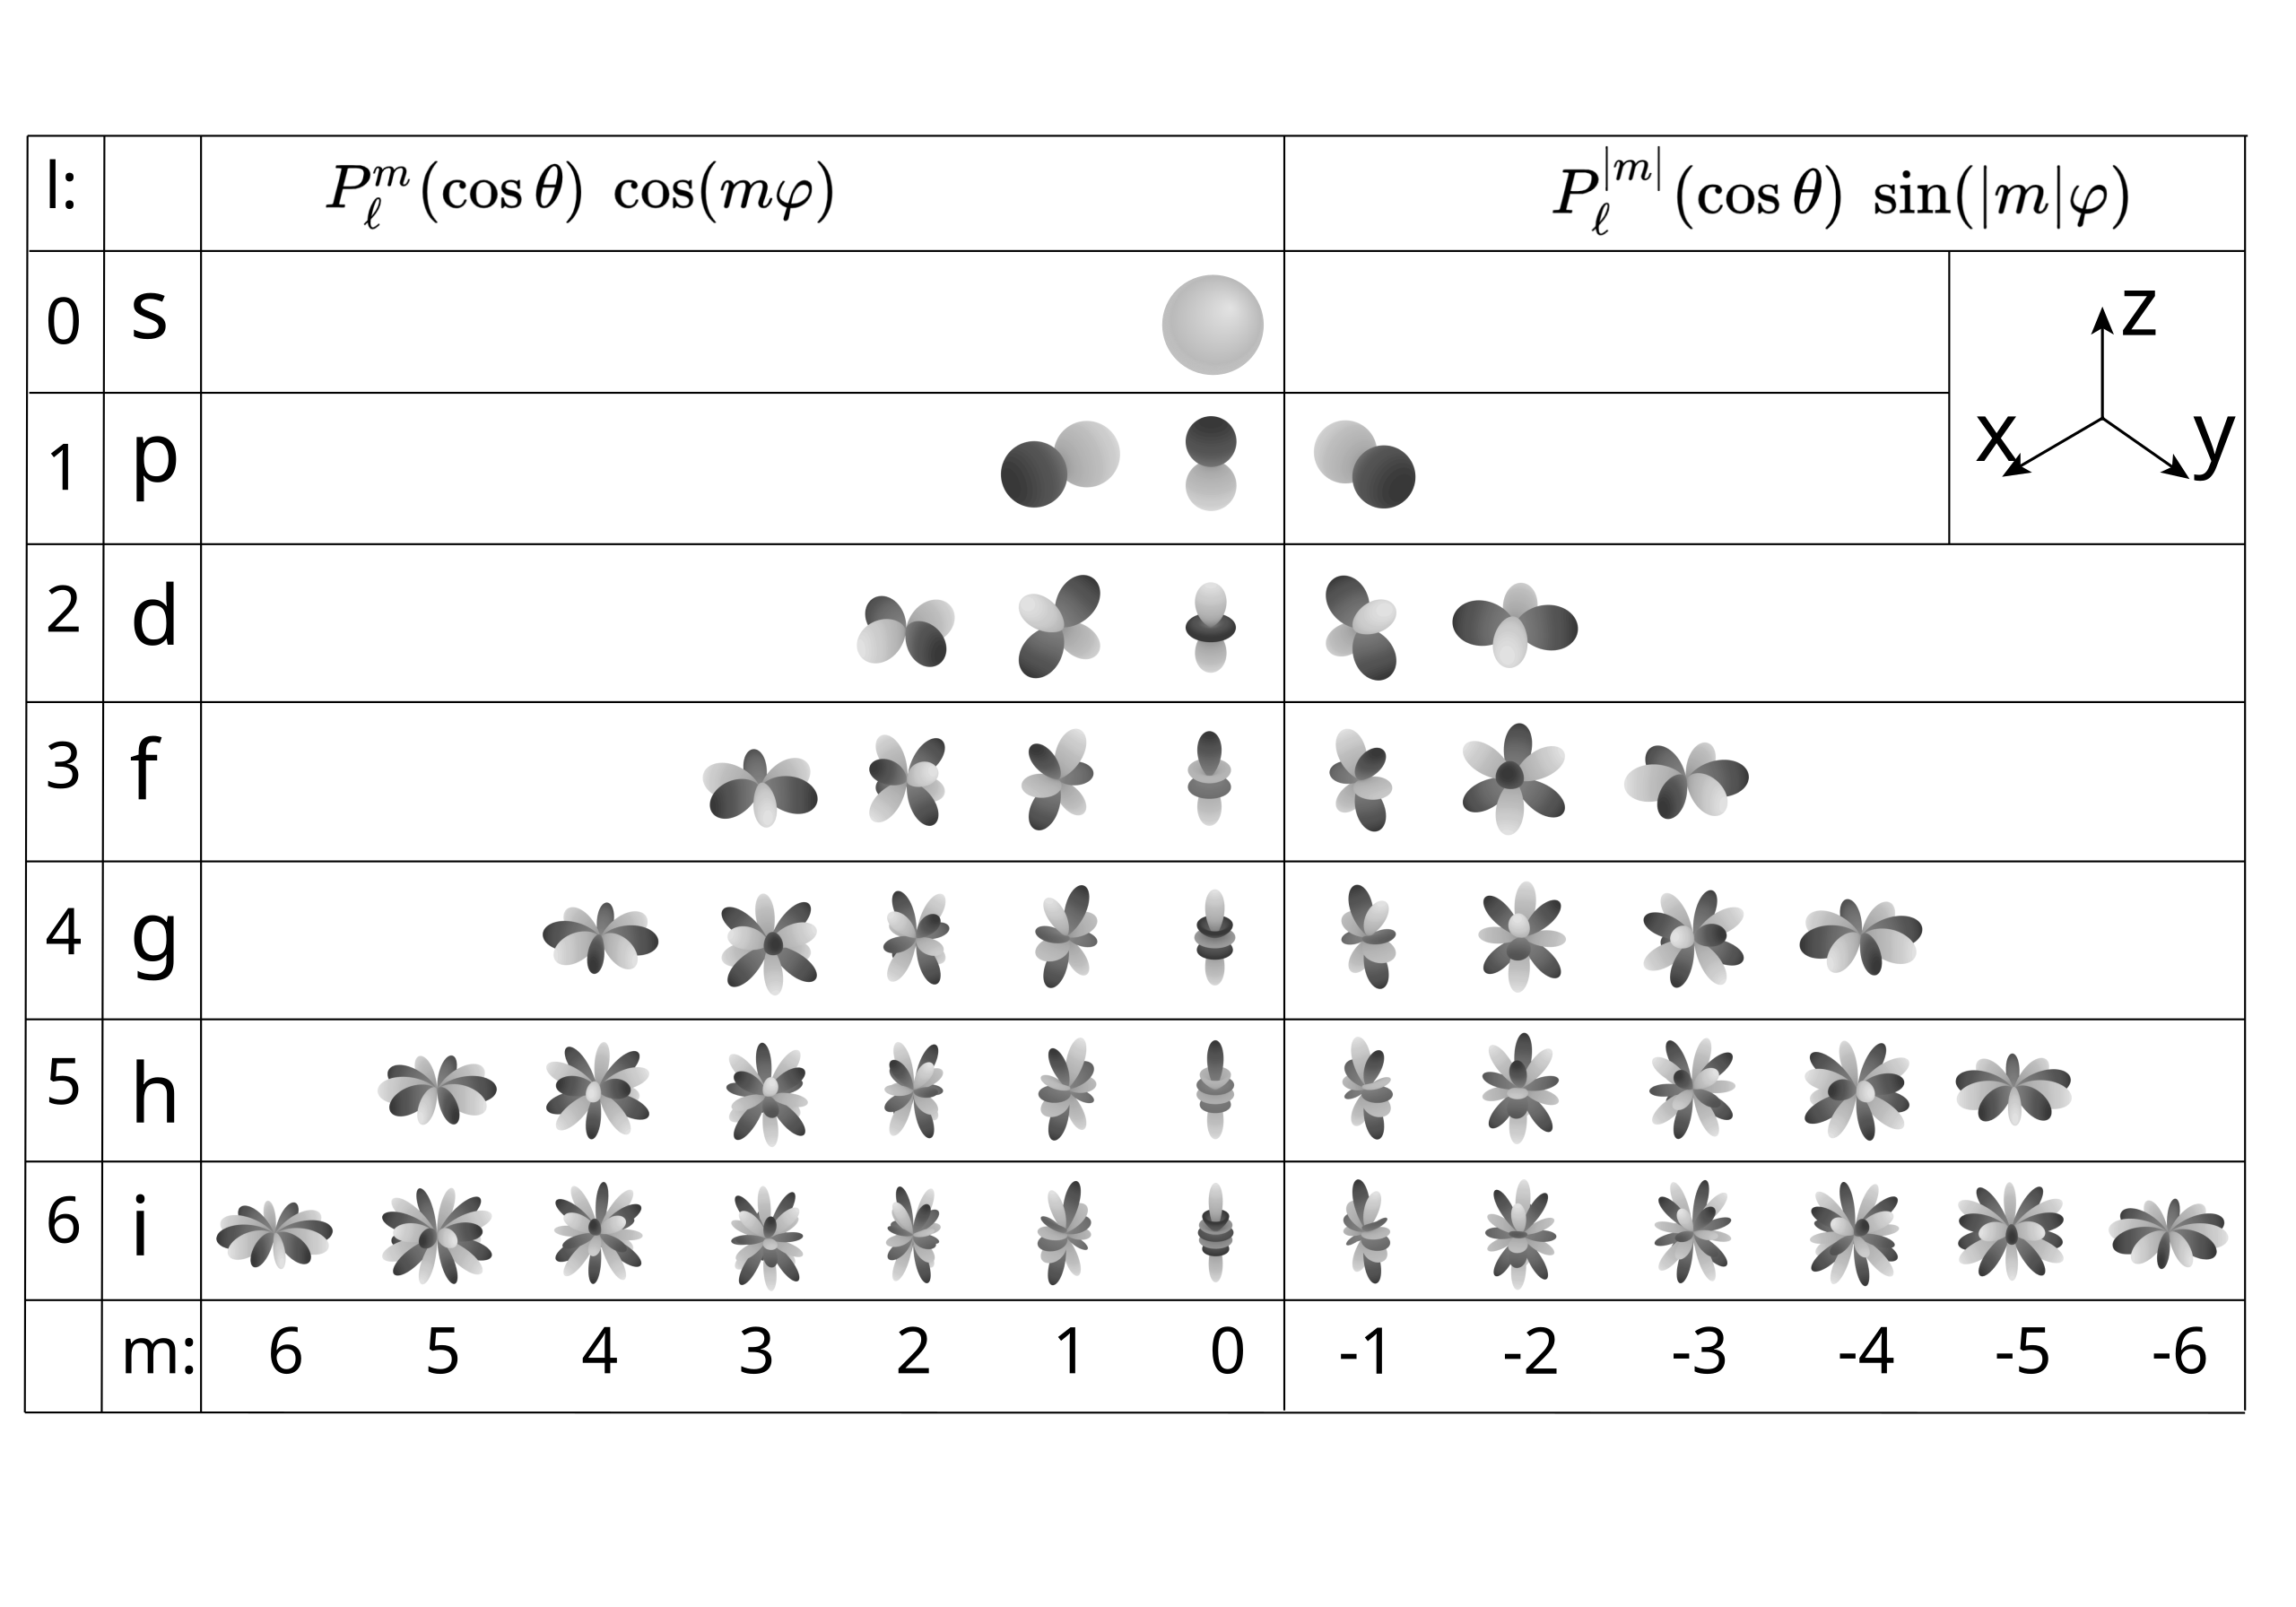
\includegraphics[height=7cm]{images/jgnn/harmonic/harmonics_ill.png}
  \caption{Illustration of the real part of the spherical harmonics}
  \label{fig:annex:jgnn:harmonic:ill}
\end{figure}

For the following analysis, we will define the \textit{Power} of an harmonic as
\begin{equation}
  S_{ff}(l) = \frac{1}{2l + 1} \sum_{m=-l}^l |a_l^m|^2
\end{equation}
and the \textit{Relative Power} as:
\begin{equation}
  P^h_l = \frac{S_{ff}(l)}{\sum_l S_{ff}(l)}
\end{equation}

For this study we will use 10k positron events with $E_{kin} \in [0; 9]$ MeV uniformly distributed in the CD from the JUNO official simulation version J23.0.1-rc8.dc1 (released the 7th January 2024). All the event are \textit{calib} level, with simulation of the physics, electronics, digitizations and triggers. We first take a sub-set of 1k events and look at the power and relative power distribution depending on the radius and harmonic degree $l$. The results are shown in figure \ref{fig:annex:jgnn:harmonic:radius_dependent}. While don't see any pattern in absolute power but it is pretty clear that we see a correlation between the relative power of $l=0$ and the radius of the event.

\begin{figure}[ht]
  \centering
  \begin{subfigure}[t]{0.48\linewidth}
    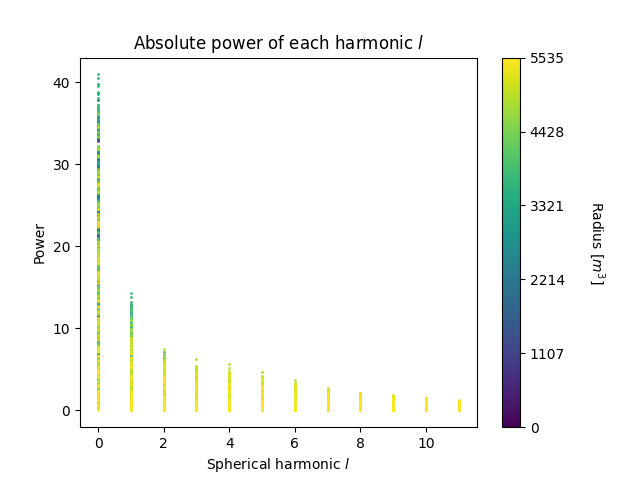
\includegraphics[width=\linewidth]{images/jgnn/harmonic/abs_power_radius_dependency.png}
  \end{subfigure}
  \hfill
  \begin{subfigure}[t]{0.48\linewidth}
    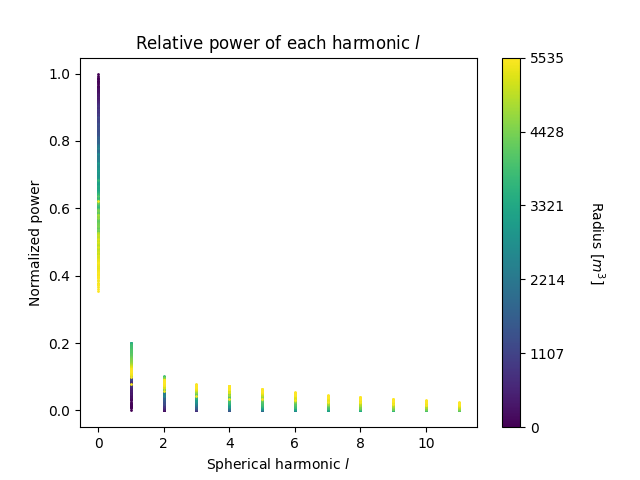
\includegraphics[width=\linewidth]{images/jgnn/harmonic/power_radius_dependency.png}
  \end{subfigure}
  \caption{Scatter plot of the absolute and relative power, respectively on the left and right plot, of each harmonic degree $l$. The color indicate the radius of the event.}
  \label{fig:annex:jgnn:harmonic:radius_dependent}
\end{figure}

When applying the same study but dependent on the energy, no clear correlation appear. The results for the $l=0$ harmonic are presented in the figure \ref{fig:annex:jgnn:harmonic:energy_dependent}. Thus, in this study we will focus on the radial dependency of the relative power of each harmonic.

In figures \ref{fig:annex:jgnn:harmonic:fit1} and \ref{fig:annex:jgnn:harmonic:fit2} are presented the distribution of the relative power of each harmonic for $l \in [0, 11]$. The relation between the radius and the relative power become even more clear, especially for the first harmonics $l \in [0, 4]$. After that for $l > 4$ their relative power is close to 0 for central event, thus loosing power. It also interesting to note the change of behavior in the TR area, clearly visible for $l = 1$ and $l = 2$.

As an erzats of reconstruction algorithm, we fit each of those distribution with a 9th degree polynomial for simplicity which give us the relation
\begin{equation}
  F(R^3) \longmapsto P^h_l
\end{equation}
We do it this way because some of the distribution have multiple solution for a given relative power, for example $l = 1$. We now \textit{just} need to find
\begin{equation}
  F^{-1}(P^h_l) \longmapsto R^3
\end{equation}
Inverting a 9th degree polynomial is hard, if not impossible. The presence of multiple roots for the same power complexify the task even more. To circumvent this problem, we reconstruct the radius by locating the minima of $(F(R^3) - \hat{P}^h_l)^2$ where $\hat{P}^h_l$ is the measured power fraction.

To distinguish between multiple possible minima, we use as a starting point the radius given by the procedure on $l = 0$ that, by looking at the fit in figure \ref{fig:annex:jgnn:harmonic:fit1}, should present only one minima. We also impose bound on the possible reconstructed $R^3$ as $R^3 \in [R^3_0 - 100, R^3_0 + 100]$ where $R^3_0$ is the reconstructed $R^3$ by the harmonic $l=0$.

The minimization algorithm used are the Bent algorithm for $l=0$ and the Bounded algorithm for $l > 0$ provided by the Scipy library \cite{virtanen_scipy_2020}. We then do the mean of the reconstructed radius from the different harmonics. The reconstruction results are shown in figure \ref{fig:annex:jgnn:harmonic:reco}. The performance seems correct but we see heavy fluctuation in the bias. To really be used as a reconstruction algorithm, the method needs to be refined as discussed in the next section.

\begin{figure}[ht]
  \centering
  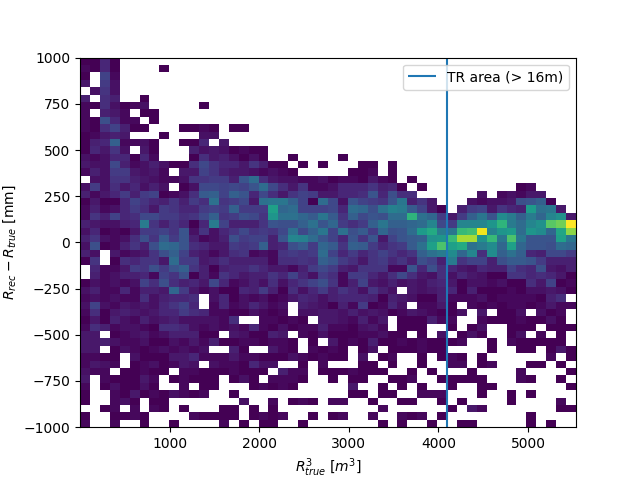
\includegraphics[height=6cm]{images/jgnn/harmonic/Radius_reco.png}
  \caption{Error on the reconstructed radius vs the true radius by the harmonic method}
  \label{fig:annex:jgnn:harmonic:reco}
\end{figure}

\section*{Conclusion}

We have clearly shown in this analysis the relevance the of relative harmonic power for radius reconstruction, and provided an erzats of a reconstruction algorithm. We will not delve further in this thesis but if we wanted to refine this algorithm multiple point need to be addressed:
\begin{itemize}
  \item No energy signature in the harmonics: This is surprising that there is no correlation between the energy and the amplitude of the harmonics. We know that the energy is heavily correlated with the total number of photoelectrons collected, it would be unintuitive that we see no relation.
  \item Localization of the event: We shown here the relation between the relative power of the harmonic and the radius but don't get any information about the $\theta$ and $\phi$ spherical coordinates. This information is probably hidden in the individual power of each order $m$ of the degree $l$. This intuition comes from the figure \ref{fig:annex:jgnn:harmonic:ill} where in the higher degree $l$ we see that the order $m$ are oriented. Intuitively, the order should be able to indicate a direction where the signal is more powerful.
  \item Combination of the degree power: Here we combined the radius reconstructed by the different degree via a simple mean but we shown in section \ref{sec:jcnn:combination} and annex \ref{sec:annex:jcnn:alpha} that this is note the optimal way to combine estimator. A more refined algorithm probably exist to take into account the predicting power of each order.
\end{itemize}

\begin{figure}
  \centering
  \begin{subfigure}[t]{0.48\linewidth}
    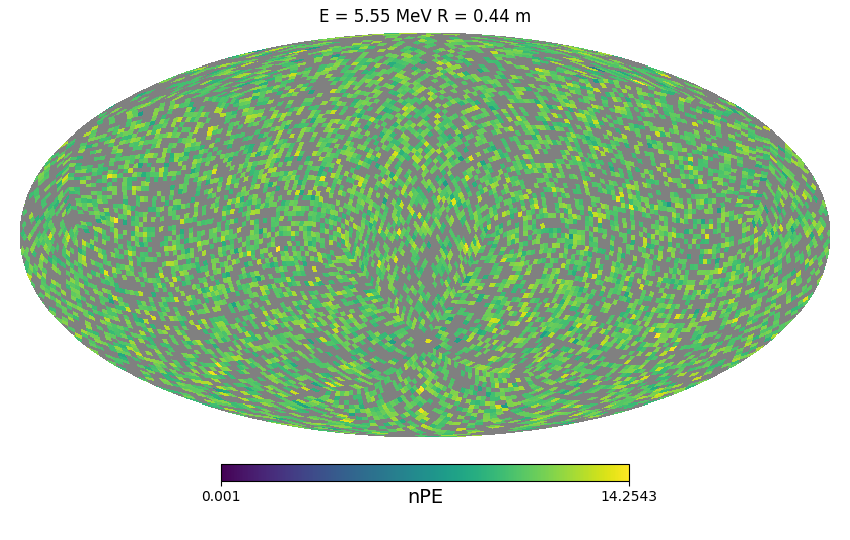
\includegraphics[width=\linewidth]{images/jgnn/harmonic/event_idx_0.png}
    \caption{}
  \end{subfigure}
  \hfill
  \begin{subfigure}[t]{0.48\linewidth}
    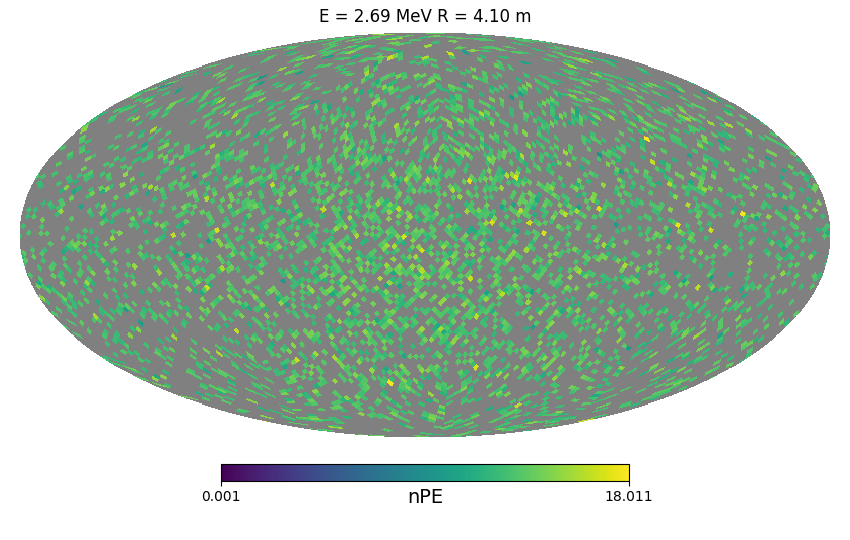
\includegraphics[width=\linewidth]{images/jgnn/harmonic/event_idx_10.png}
    \caption{}
  \end{subfigure}


  \begin{subfigure}[t]{0.48\linewidth}
    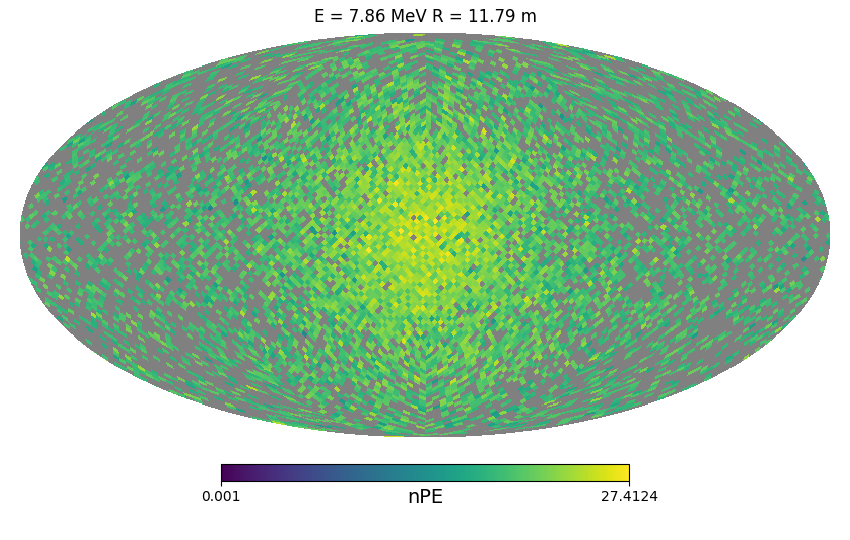
\includegraphics[width=\linewidth]{images/jgnn/harmonic/event_idx_300.png}
    \caption{}
  \end{subfigure}
  \hfill
  \begin{subfigure}[t]{0.48\linewidth}
    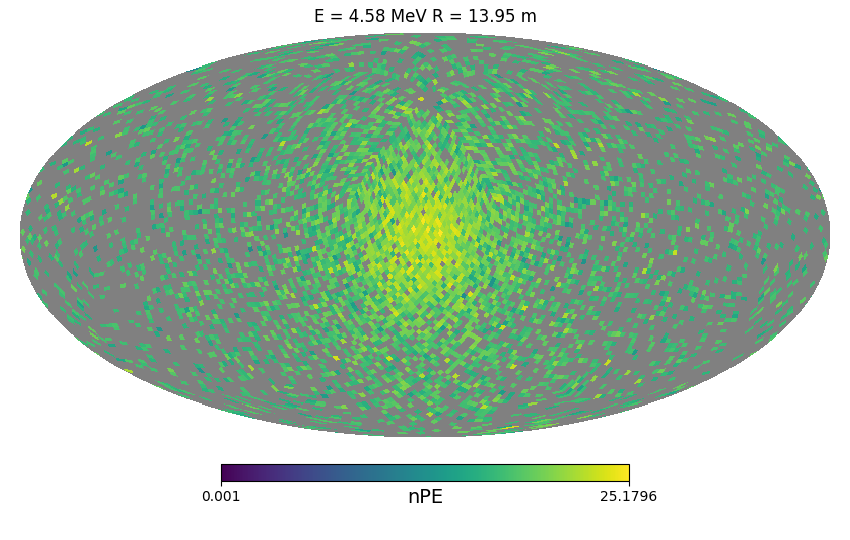
\includegraphics[width=\linewidth]{images/jgnn/harmonic/event_idx_500.png}
    \caption{}
  \end{subfigure}


  \begin{subfigure}[t]{0.48\linewidth}
    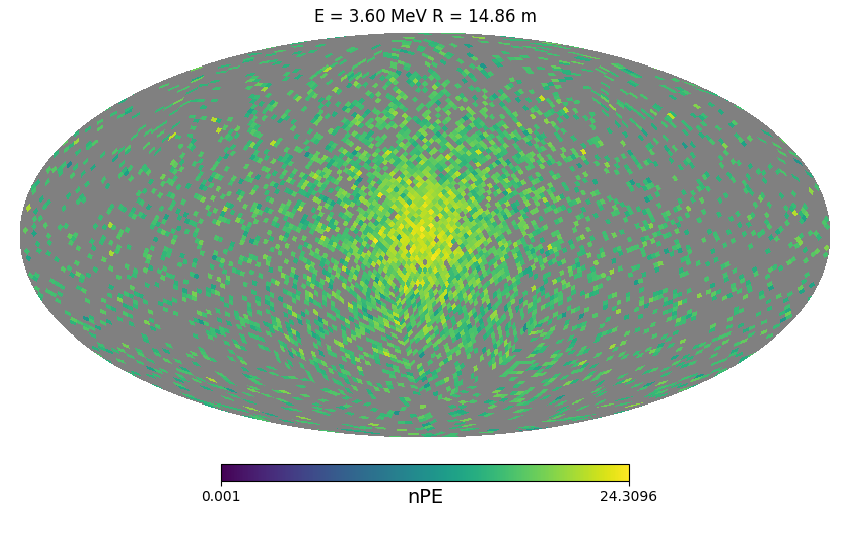
\includegraphics[width=\linewidth]{images/jgnn/harmonic/event_idx_600.png}
    \caption{}
  \end{subfigure}
  \hfill
  \begin{subfigure}[t]{0.48\linewidth}
    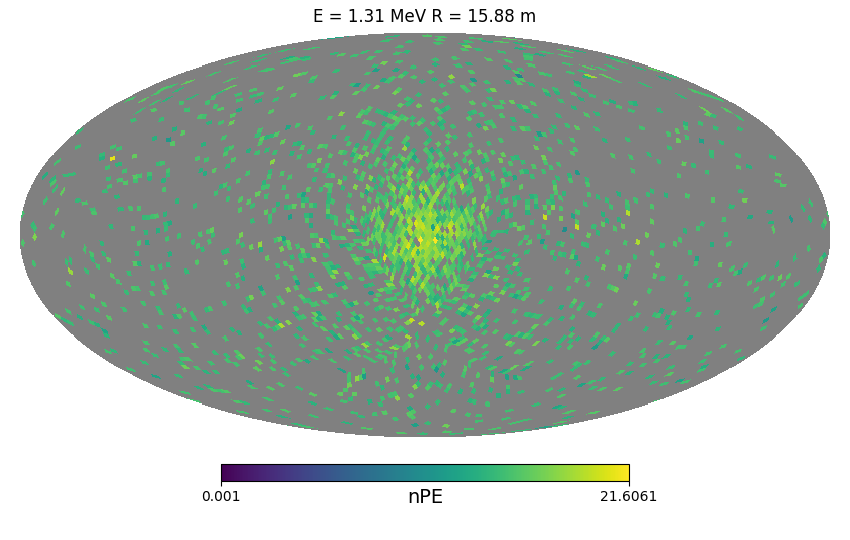
\includegraphics[width=\linewidth]{images/jgnn/harmonic/event_idx_700.png}
    \caption{}
  \end{subfigure}



  \begin{subfigure}[t]{0.48\linewidth}
    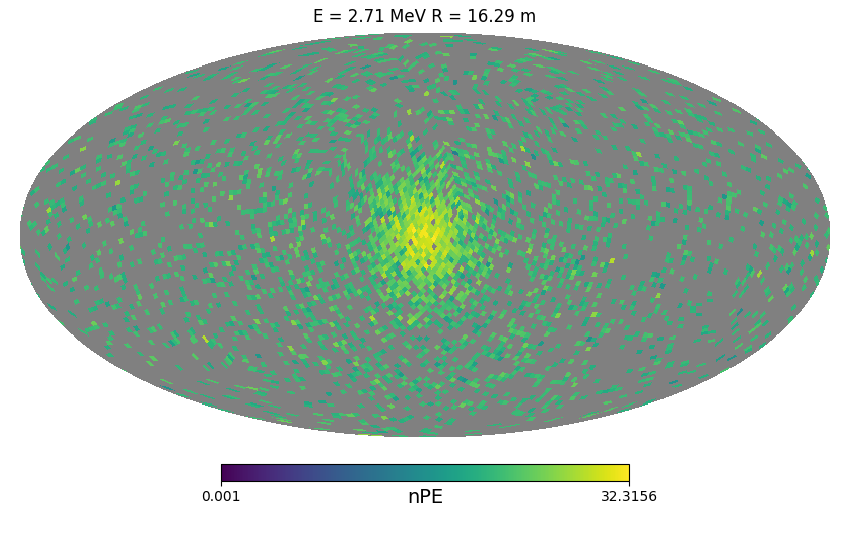
\includegraphics[width=\linewidth]{images/jgnn/harmonic/event_idx_750.png}
    \caption{}
  \end{subfigure}
  \hfill
  \begin{subfigure}[t]{0.48\linewidth}
    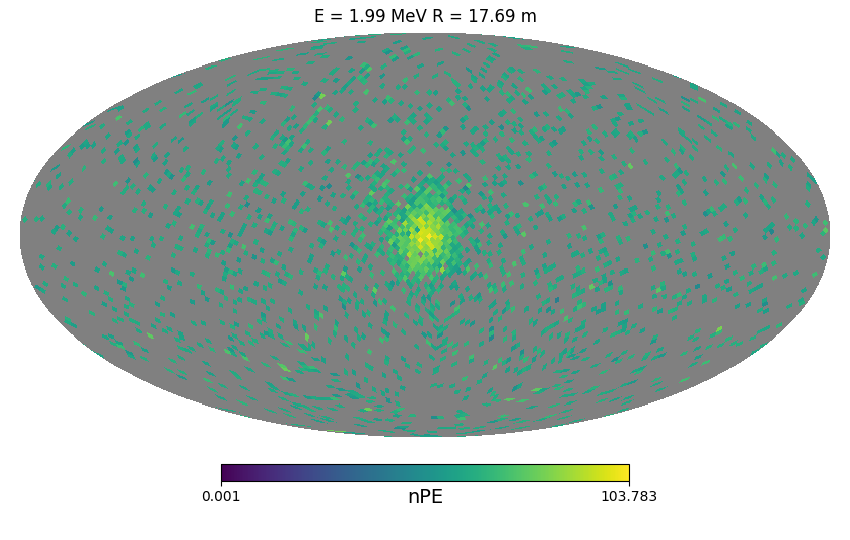
\includegraphics[width=\linewidth]{images/jgnn/harmonic/event_idx_999.png}
    \caption{}
  \end{subfigure}

  \caption{Charge repartition in JUNO as seen by the Healpix segmentation. Those are Healpix map of order 5 (i.e. 12288 pixels). The color represent the summed charge of the PMTs in each pixels. The color scale is logarithmic. The view have been centered to prevent event deformations.}
  \label{fig:annex:jgnn:harmonic:events}
\end{figure}

\begin{figure}[ht]
  \centering
  \begin{subfigure}[t]{0.48\linewidth}
    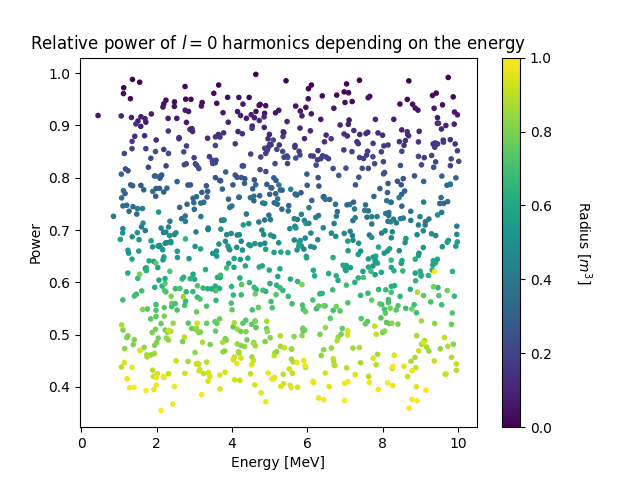
\includegraphics[width=\linewidth]{images/jgnn/harmonic/power_energy_dependency.png}
  \end{subfigure}
  \hfill
  \begin{subfigure}[t]{0.48\linewidth}
    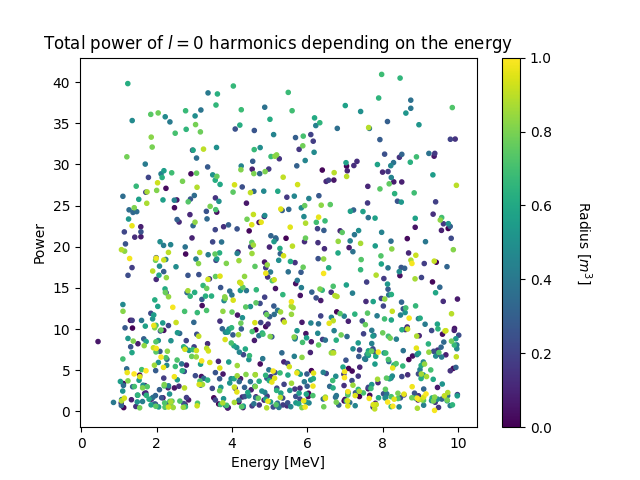
\includegraphics[width=\linewidth]{images/jgnn/harmonic/rel_power_energy_dependency.png}
  \end{subfigure}
  \caption{Scatter plot of the absolute and relative power, respectively on the left and right plot, of the $l=0$ harmonic. The color indicate the radius of the event.}
  \label{fig:annex:jgnn:harmonic:energy_dependent}
\end{figure}

\begin{figure}[ht]
  \centering
  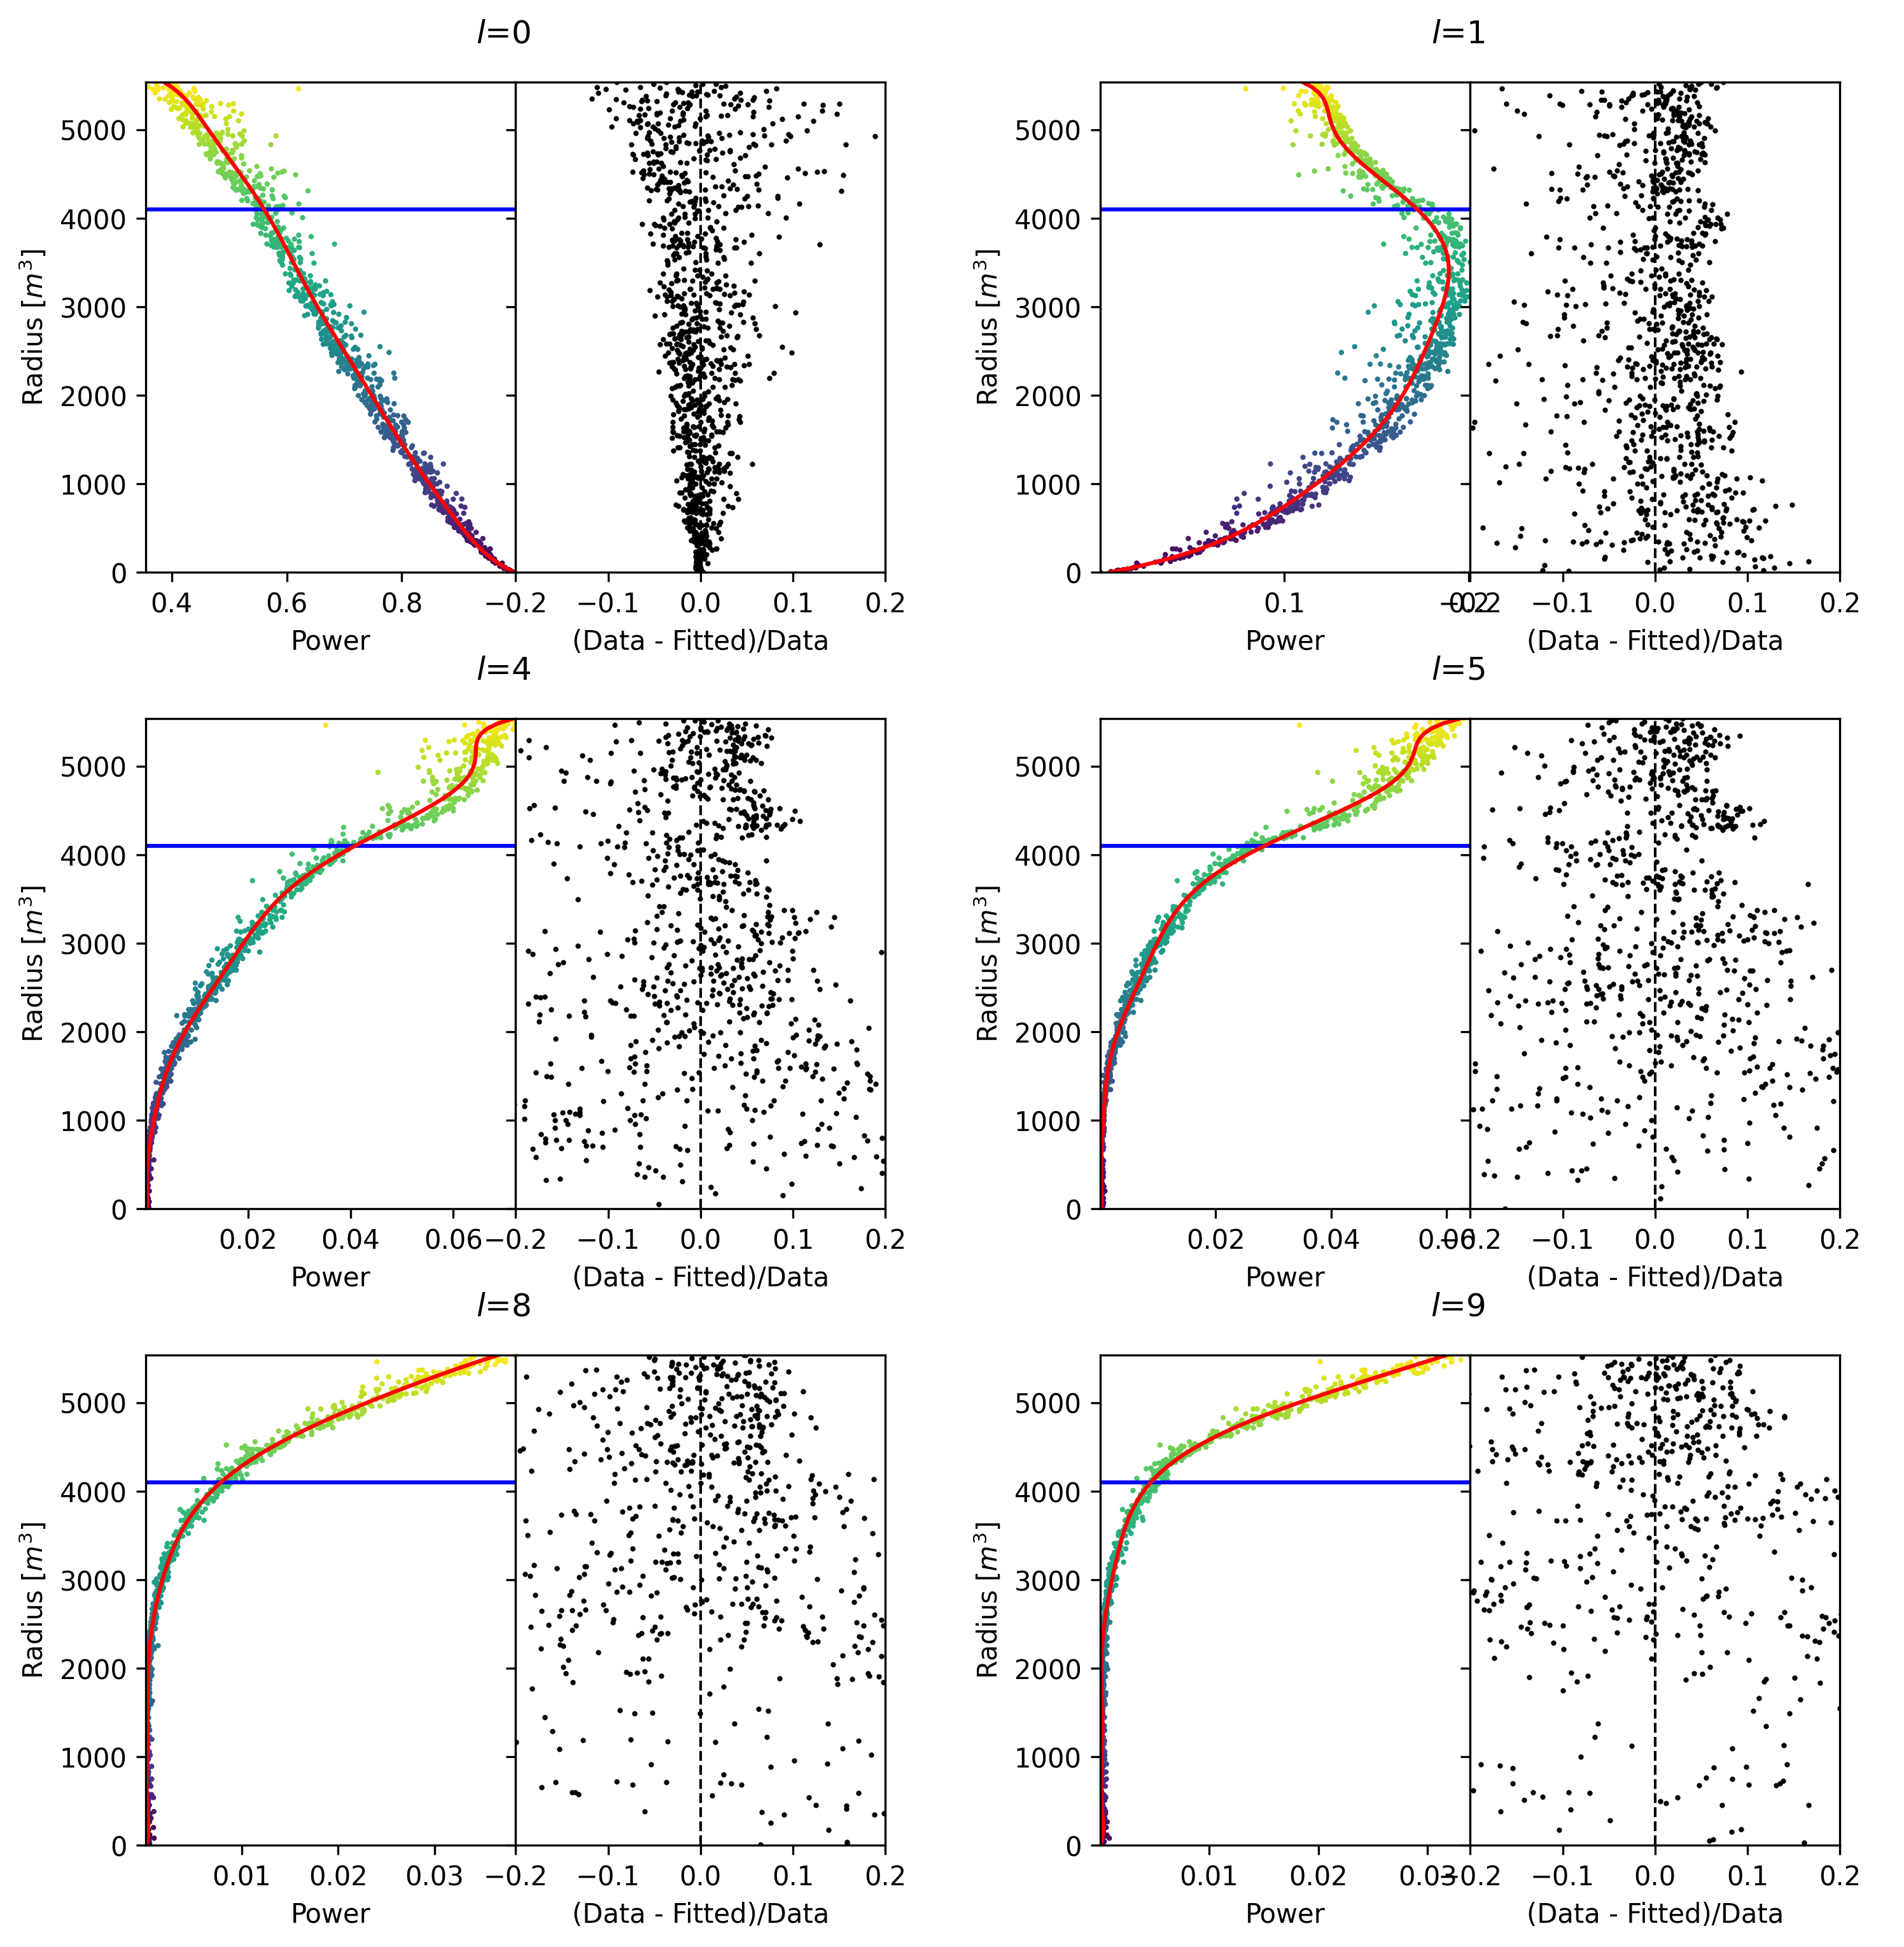
\includegraphics[width=\linewidth]{images/jgnn/harmonic/power_fit.png}
  \caption{Plot of the distribution of the relative power of each harmonic dependent on $R^3$ (on the left). The Total Reflection (TR) area is represented by the horizontal blue line. The distribution are fitted using a 9th degree polynomial (red curve). The relative power error between the distribution and the fit is represented on the left. \textbf{Part 1}}
  \label{fig:annex:jgnn:harmonic:fit1}
\end{figure}
\begin{figure}[ht]
  \centering
  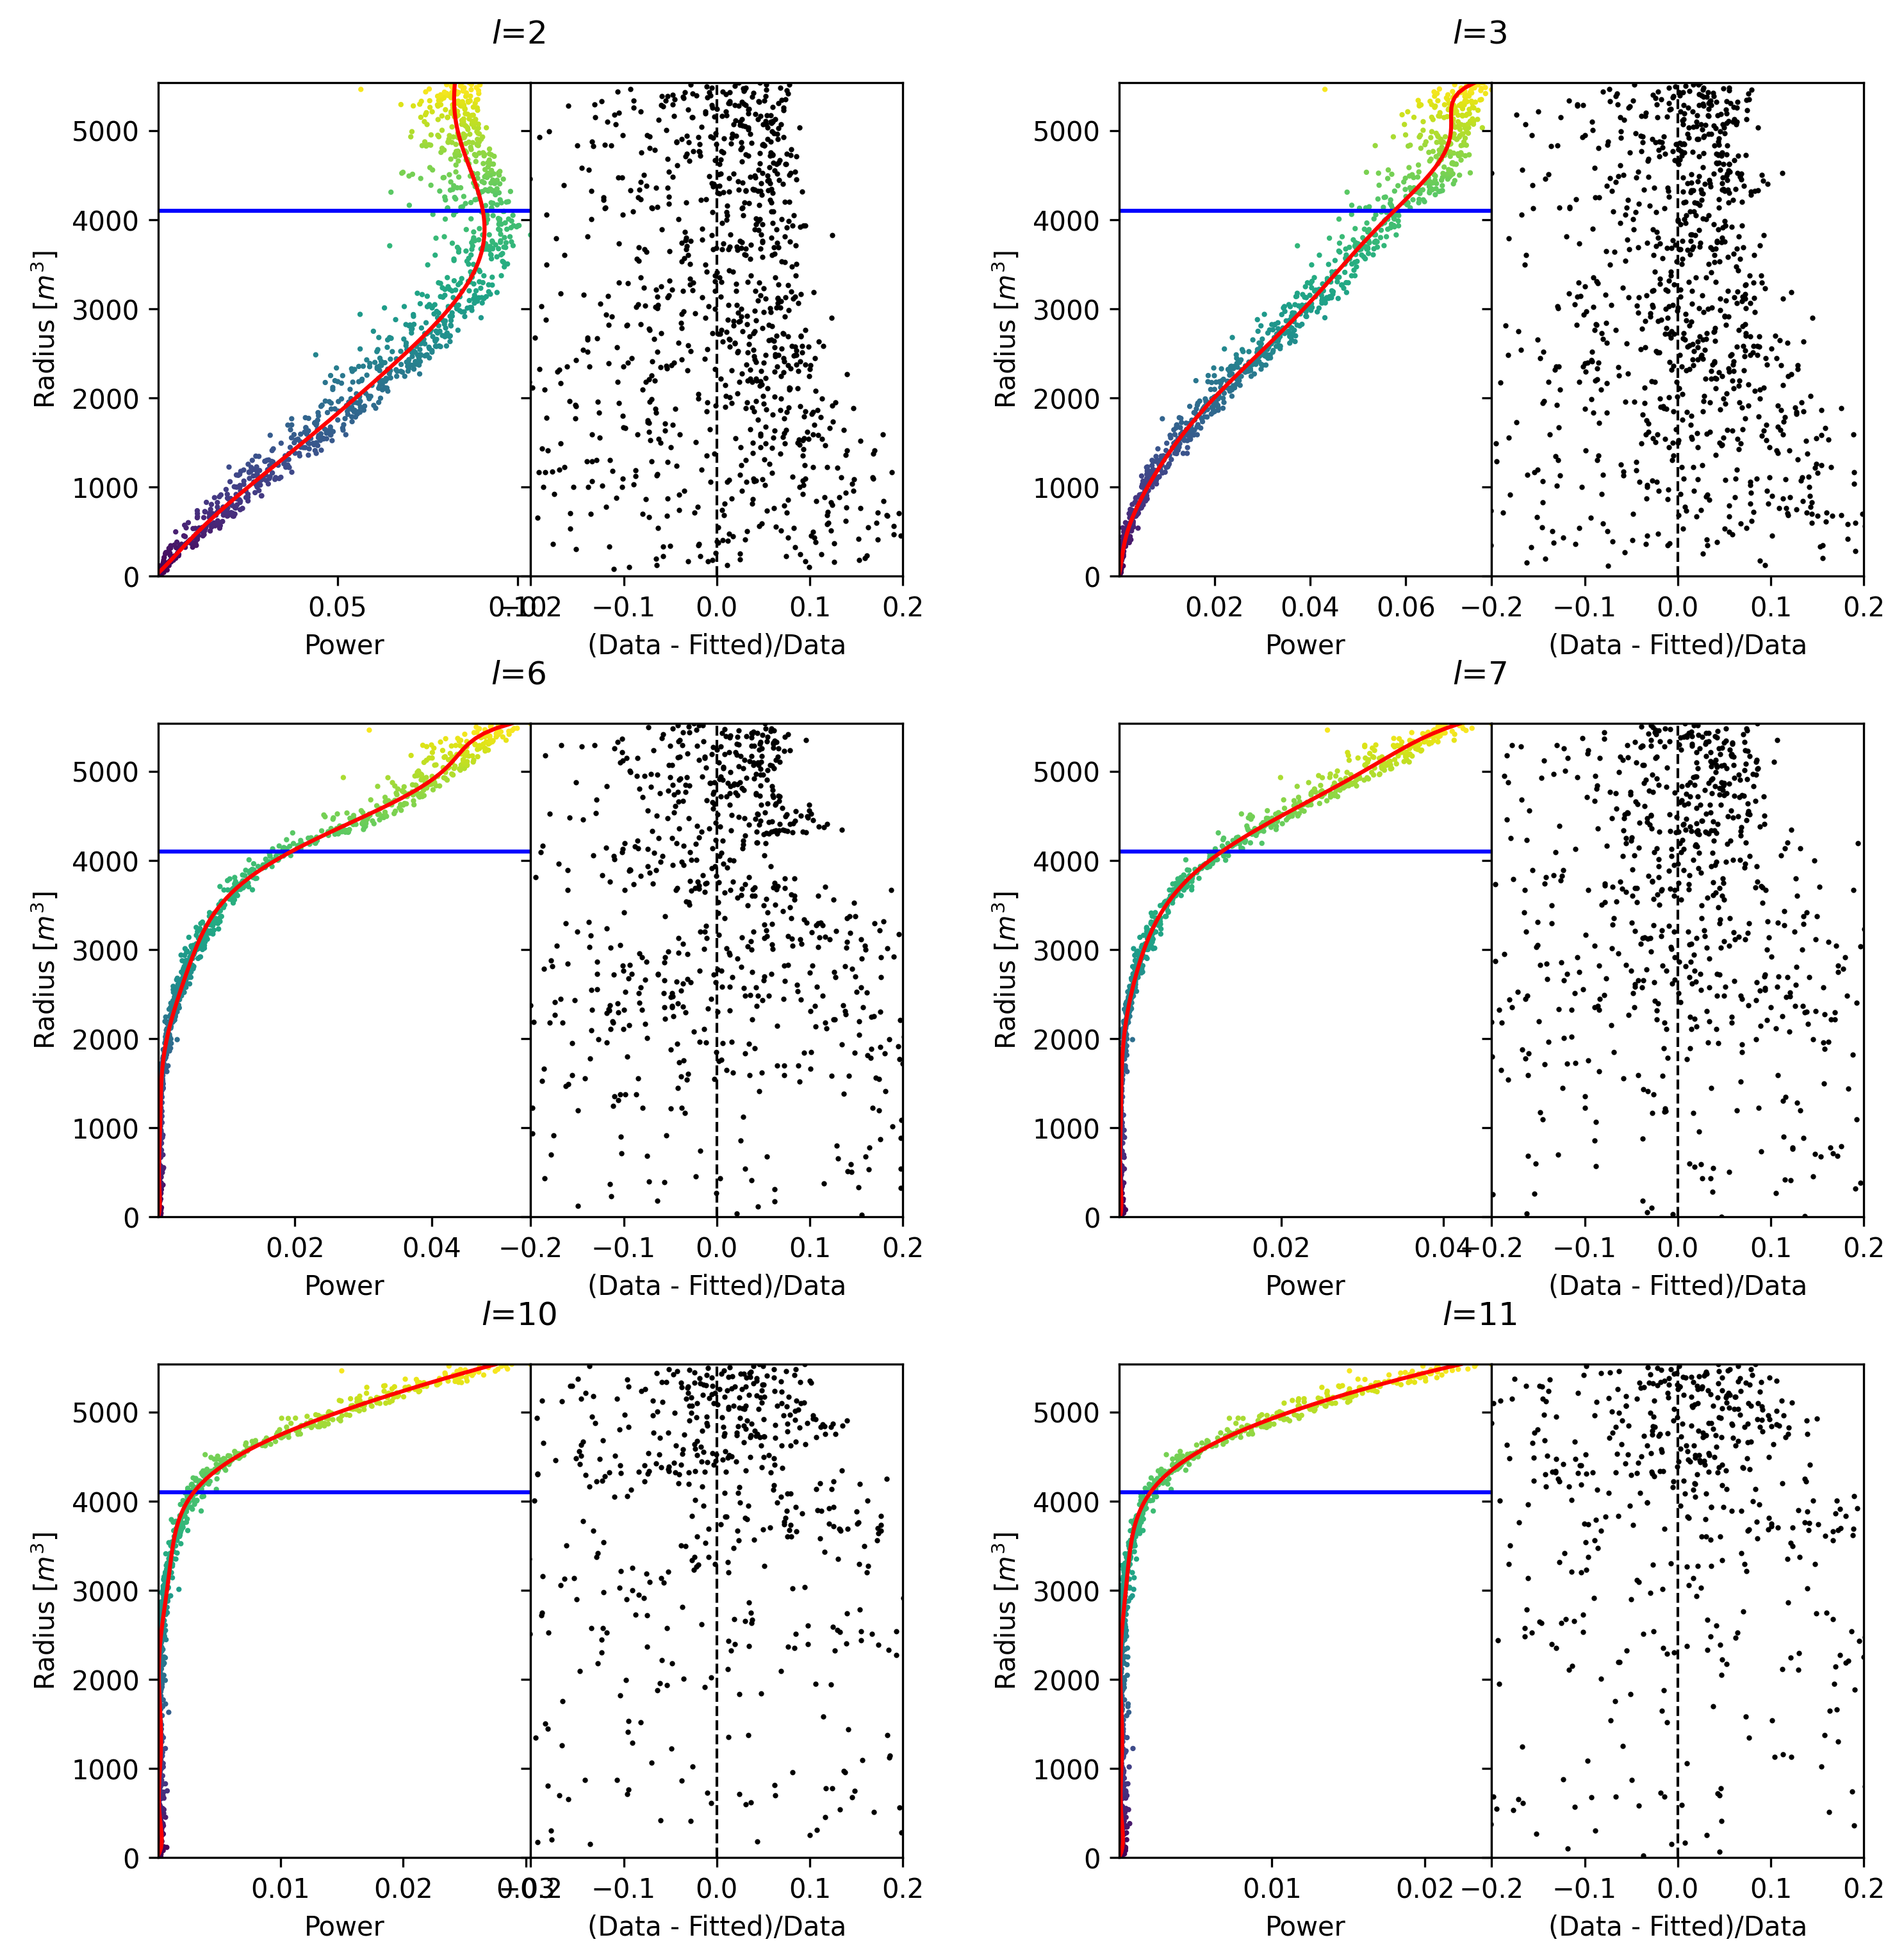
\includegraphics[width=\linewidth]{images/jgnn/harmonic/power_fit_pt2.png}
  \caption{Plot of the distribution of the relative power of each harmonic dependent on $R^3$ (on the left). The Total Reflection (TR) area is represented by the horizontal blue line. The distribution are fitted using a 9th degree polynomial (red curve). The relative power error between the distribution and the fit is represented on the left. \textbf{Part 2}}
  \label{fig:annex:jgnn:harmonic:fit2}
\end{figure}

\end{document}
